\appendix

尽管合成数据集能够提供带有真实深度标注的大规模训练数据，但许多数据集存在质量问题，例如无效背景、空间错位、裁剪伪影以及错误的深度值，这些问题可能影响模型训练。因此，我们进行了仔细的预处理，以过滤有问题的样本并裁剪不切实际的深度范围，确保为我们的教师模型提供高质量的监督。
\section{数据处理}

为了训练教师模型，我们对以下原始训练数据集进行了如下预处理。

\paragraph{TartanAir.} 我们在训练中移除了{\tt amusement}场景，因为该场景存在无效背景（天空盒）（图~\ref{fig:tartanair_problem}）。我们将{\tt carwelding}、{\tt hospital}、{\tt ocean}、{\tt office}和{\tt office2}场景的最大深度值分别裁剪为80、30、1000、30和30。

\begin{figure}[h]
    \centering
    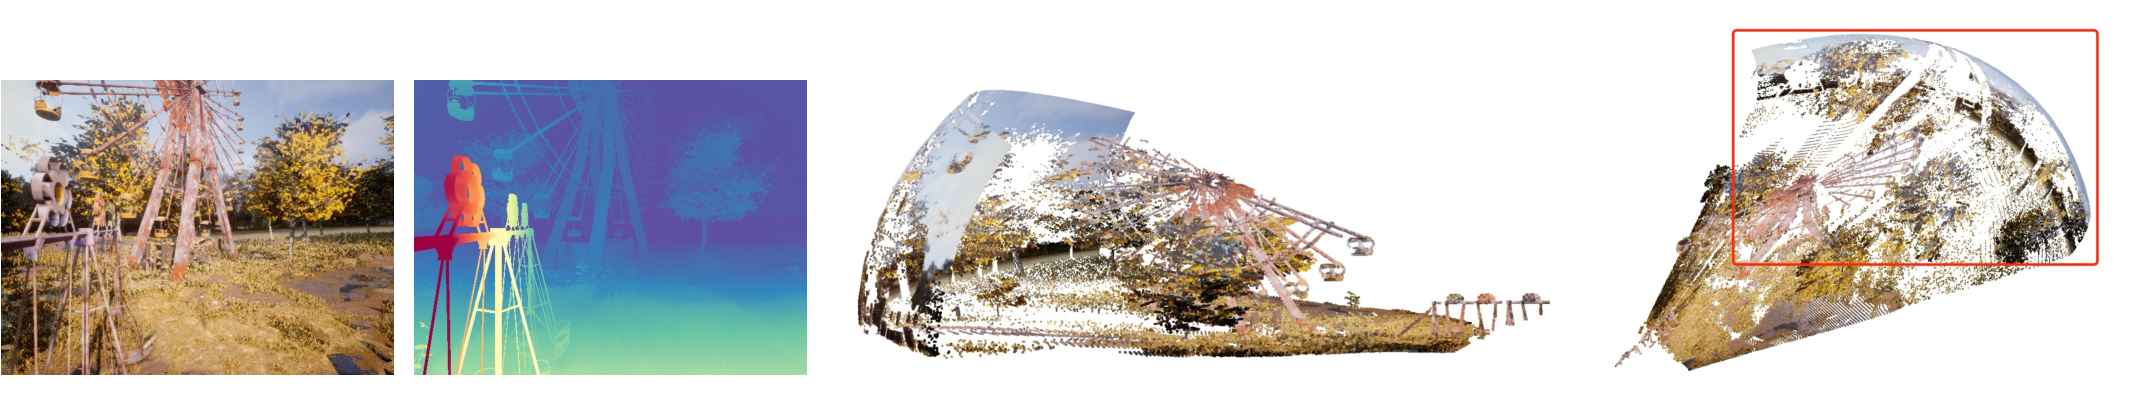
\includegraphics[width=1\linewidth]{figs/pdfs/tartanair_problem.pdf}
    \caption{\textbf{TartanAir数据集中{\tt amusement}场景的无效背景。}}
    \label{fig:tartanair_problem}
\end{figure}

\paragraph{IRS.} 我们注意到IRS中的部分场景在图像与深度图之间存在空间错位（图~\ref{fig:irs_problem}）。为过滤这些图像-深度错位的样本，我们首先在图像（转换为灰度图）和深度图上运行Canny边缘检测器以提取边界。接着，我们将边界膨胀1个像素，并计算图像边界与深度边界之间的交集百分比。然后，我们再将边界膨胀3个像素，并计算图像边界与深度边界之间的交集。最后，计算两个交集之间的比率，并移除比率低于某一阈值的样本。

\begin{figure}[h]
    \centering
    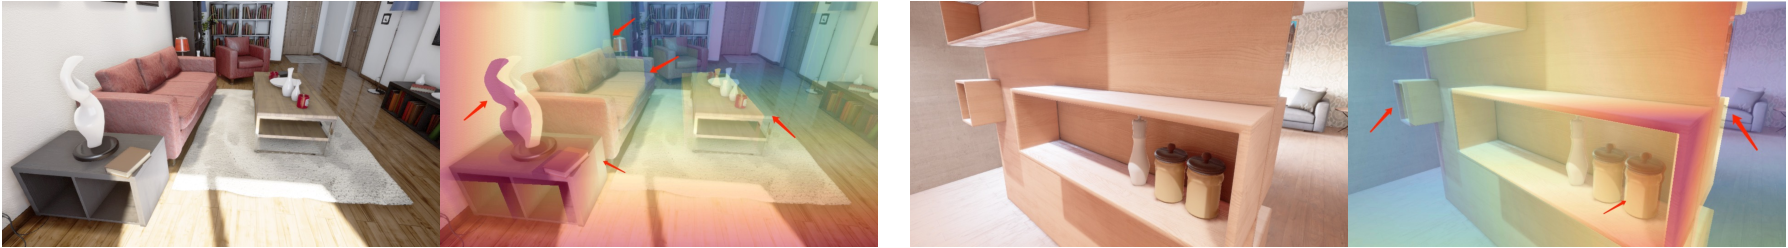
\includegraphics[width=1.0\linewidth]{figs/pdfs/irs_problem.pdf}
    \caption{\textbf{IRS数据集中的图像-深度空间错位。}}
    \label{fig:irs_problem}
\end{figure}

\paragraph{UnrealStereo4K.} 我们移除了包含大面积错误区域的{\tt 00003}场景。我们还移除了存在裁剪问题的{\tt 00004}场景。对于{\tt 00008}场景，我们移除了海洋区域没有深度值的样本（图像编号9-13、23-29、80-82、86-88、96、103-111、126-136、144-145、148-154、173-176、178-179、186-187、191-192、198-199）（图~\ref{fig:unrealstereo4k_problem}）。

\begin{figure}[h]
    \centering
    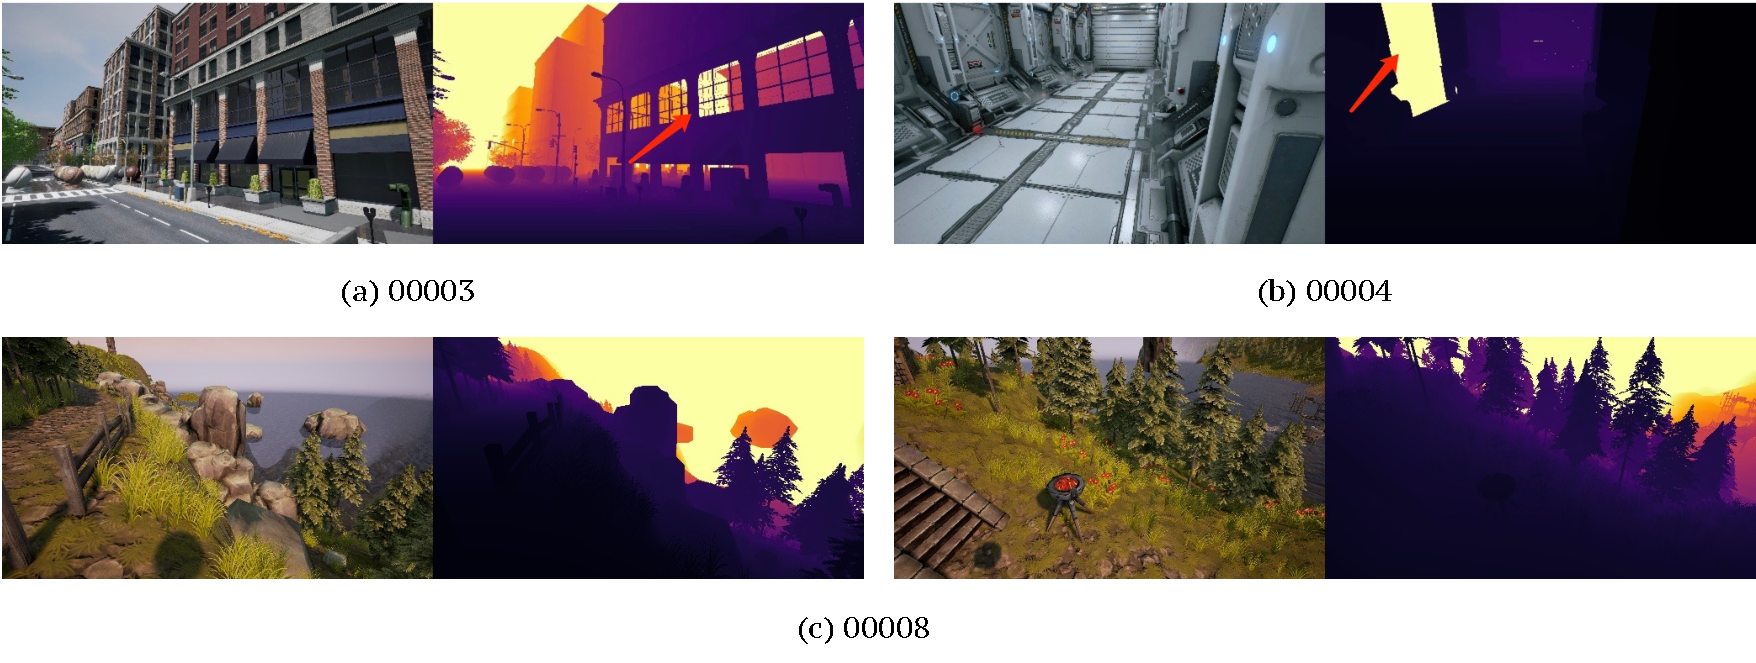
\includegraphics[width=1.0\linewidth]{figs/pdfs/unrealstereo4k_problem1.pdf}
    \caption{\textbf{UnrealStereo4K数据集中的错误样本。}{\tt 00003}场景中的窗户是透明的；{\tt 00004}场景存在裁剪问题；{\tt 00008}场景中海洋区域没有深度值。}
    \label{fig:unrealstereo4k_problem}
\end{figure}

\paragraph{GTA-SfM.} 我们将最大深度值裁剪为1000。

\paragraph{Kenburns.} 根据GitHub问题\footnote{\url{https://github.com/sniklaus/3d-ken-burns/issues/40}}，我们将深度值裁剪为50,000。

\paragraph{PointOdyssey.} 我们移除了{\tt animal2\_s}和{\tt dancingroom3\_3rd}两个场景，这些场景的地面深度不正确\footnote{\url{https://github.com/y-zheng18/point_odyssey/issues/6}}。

\paragraph{TRELLIS.} 我们移除了所有后缀为{\tt stl}、{\tt abc}、{\tt STL}、{\tt PLY}、{\tt ply}的样本，因为我们注意到这些样本不包含纹理。

\paragraph{OmniObject3D.} 我们将最大深度值裁剪为10。
